\documentclass[11pt]{article}
\usepackage[margin=1in]{geometry}          
\usepackage{graphicx}
\usepackage{listings}
\usepackage[T1]{fontenc}
\usepackage[american]{babel}
\usepackage{fancyvrb}
\usepackage{bm}
\usepackage[svgnames]{xcolor}
\usepackage{amsthm, amsmath, amssymb}
\usepackage{setspace}\onehalfspacing
\usepackage[loose,nice]{units} %replace "nice" by "ugly" for units in upright fractions
 
\title{Spatio-temporal Data Analysis HW1}
\author{2020311198 Dongook Son}
\date{Spring 2020}

\lstset{% setup listings
  language=R,% set programming language
  basicstyle=\ttfamily\small,% basic font style
  backgroundcolor=\color{WhiteSmoke},
  keywordstyle=\color{blue},% keyword style
  commentstyle=\color{gray},% comment style
  numbers=left,% display line numbers on the left side
  numberstyle=\scriptsize,% use small line numbers
  numbersep=10pt,% space between line numbers and code
  tabsize=3,% sizes of tabs
  showstringspaces=false,% do not replace spaces in strings by a certain character
  captionpos=b,% positioning of the caption below
  breaklines=true,% automatic line breaking
  escapeinside={(*}{*)},% escaping to LaTeX
  fancyvrb=true,% verbatim code is typset by listings
  extendedchars=false,% prohibit extended chars (chars of codes 128--255)
  literate={"}{{\texttt{"}}}1{<-}{{$\bm\leftarrow$}}1{<<-}{{$\bm\twoheadleftarrow$}}1
  {~}{{$\bm\sim$}}1{<=}{{$\bm\le$}}1{>=}{{$\bm\ge$}}1{!=}{{$\bm\neq$}}1{^}{{$^{\bm\wedge}$}}1,% item to replace, text, length of chars
  alsoletter={.<-},% becomes a letter
  alsoother={$},% becomes other
  otherkeywords={!=, ~, $, \&, \%/\%, \%*\%, \%\%, <-, <<-, /},% other keywords
  deletekeywords={c}% remove keywords
}

\begin{document}
\maketitle

\section*{Q1}
\subsection*{(a)}
Prove $E(Y)=E(\mu+LZ)$ and $V(Y)=V(\mu+LZ)$

\begin{proof}
  \begin{align*}
    E(Y) &= E(\mu + LZ) \\
    &= \mu+E(LZ) \\
    &= \mu+LE(Z) & \text{(linearity property)} \\
    &= \mu \\
    V(Y) &= E([(Y-E(Y))(Y-E(Y))']) \\
    &= E([(Y-\mu)(Y-\mu)']) \\
    &= E([(LZ)(LZ)']) \\
    &= E([LZZ'L']) \\
    &= LE(ZZ')L' \\
    &= LV(Z)L' \\
    &= LIL' \\
    &= LL' \\
    &= \Sigma
  \end{align*}
\end{proof}

\subsection*{(b)}

\begin{lstlisting}
  create_multivariate_normal <- function (mu, Sigma) {
  lower_triangle_matrix <- t(chol(Sigma))
  dimension <- nrow(Sigma)
  Z <- rmvnorm(n = 1, mean = rep(0, dimension), sigma = diag(dimension))
  Y = mu + lower_triangle_matrix %*% Z
  return(Y)
}
\end{lstlisting}
\subsection*{(c)}
 \begin{lstlisting}
library(mvtnorm)
library(clusterGeneration)
library(yarrr)
generate_z <- function(dimension, seed= 1) {
  set.seed(seed)
  Z <- rmvnorm(n = 1, mean = rep(0, dimension), sigma = diag(dimension))
  return(Z)
}

generate_multivariate_normal_with_Z <- function (mu, Sigma, Z, seed=1) {
  set.seed(seed)
  lower_triangle_matrix <- t(chol(Sigma))
  Y = mu + (lower_triangle_matrix %*% t(Z))
  return(Y)
}


dimension <- 100
Z_sample <- generate_z(dimension)

plot(x=1,
     type="n",
     xlim = c(1,100),
     ylim = c(-10,10),
     pch = 16,
     xlab="Sample Index",
     ylab="Y_sample",
     )
grid()

set.seed(1)
Sigma <- genPositiveDefMat(dimension, covMethod="eigen")$Sigma
Y_sample <- generate_multivariate_normal_with_Z(mu = rep(0,100), Sigma = Sigma, Z = Z_sample)
points(1:100, Y_sample,
       pch = 16,
       col = transparent("coral2", trans.val = .8))

set.seed(1)
Sigma <- genPositiveDefMat(dimension, covMethod="onion")$Sigma
Y_sample <- generate_multivariate_normal_with_Z(mu = rep(0,100), Sigma = Sigma, Z = Z_sample)
points(1:100, Y_sample,
       pch = 16,
       col = transparent("coral", trans.val = .5))

set.seed(1)
Sigma <- genPositiveDefMat(dimension, covMethod="unifcorrmat")$Sigma
Y_sample <- generate_multivariate_normal_with_Z(mu = rep(0,100), Sigma = Sigma, Z = Z_sample)
points(1:100, Y_sample,
       pch = 16,
       col = transparent("coral3", trans.val = .3))

Sigma <- diag(dimension)
Y_sample <- generate_multivariate_normal_with_Z(mu = rep(0,100), Sigma = Sigma, Z = Z_sample)
points(1:100, Y_sample,
       pch = 12,
       col = transparent("blue", trans.val = .1))
\end{lstlisting}

\begin{figure}[h!]
\center{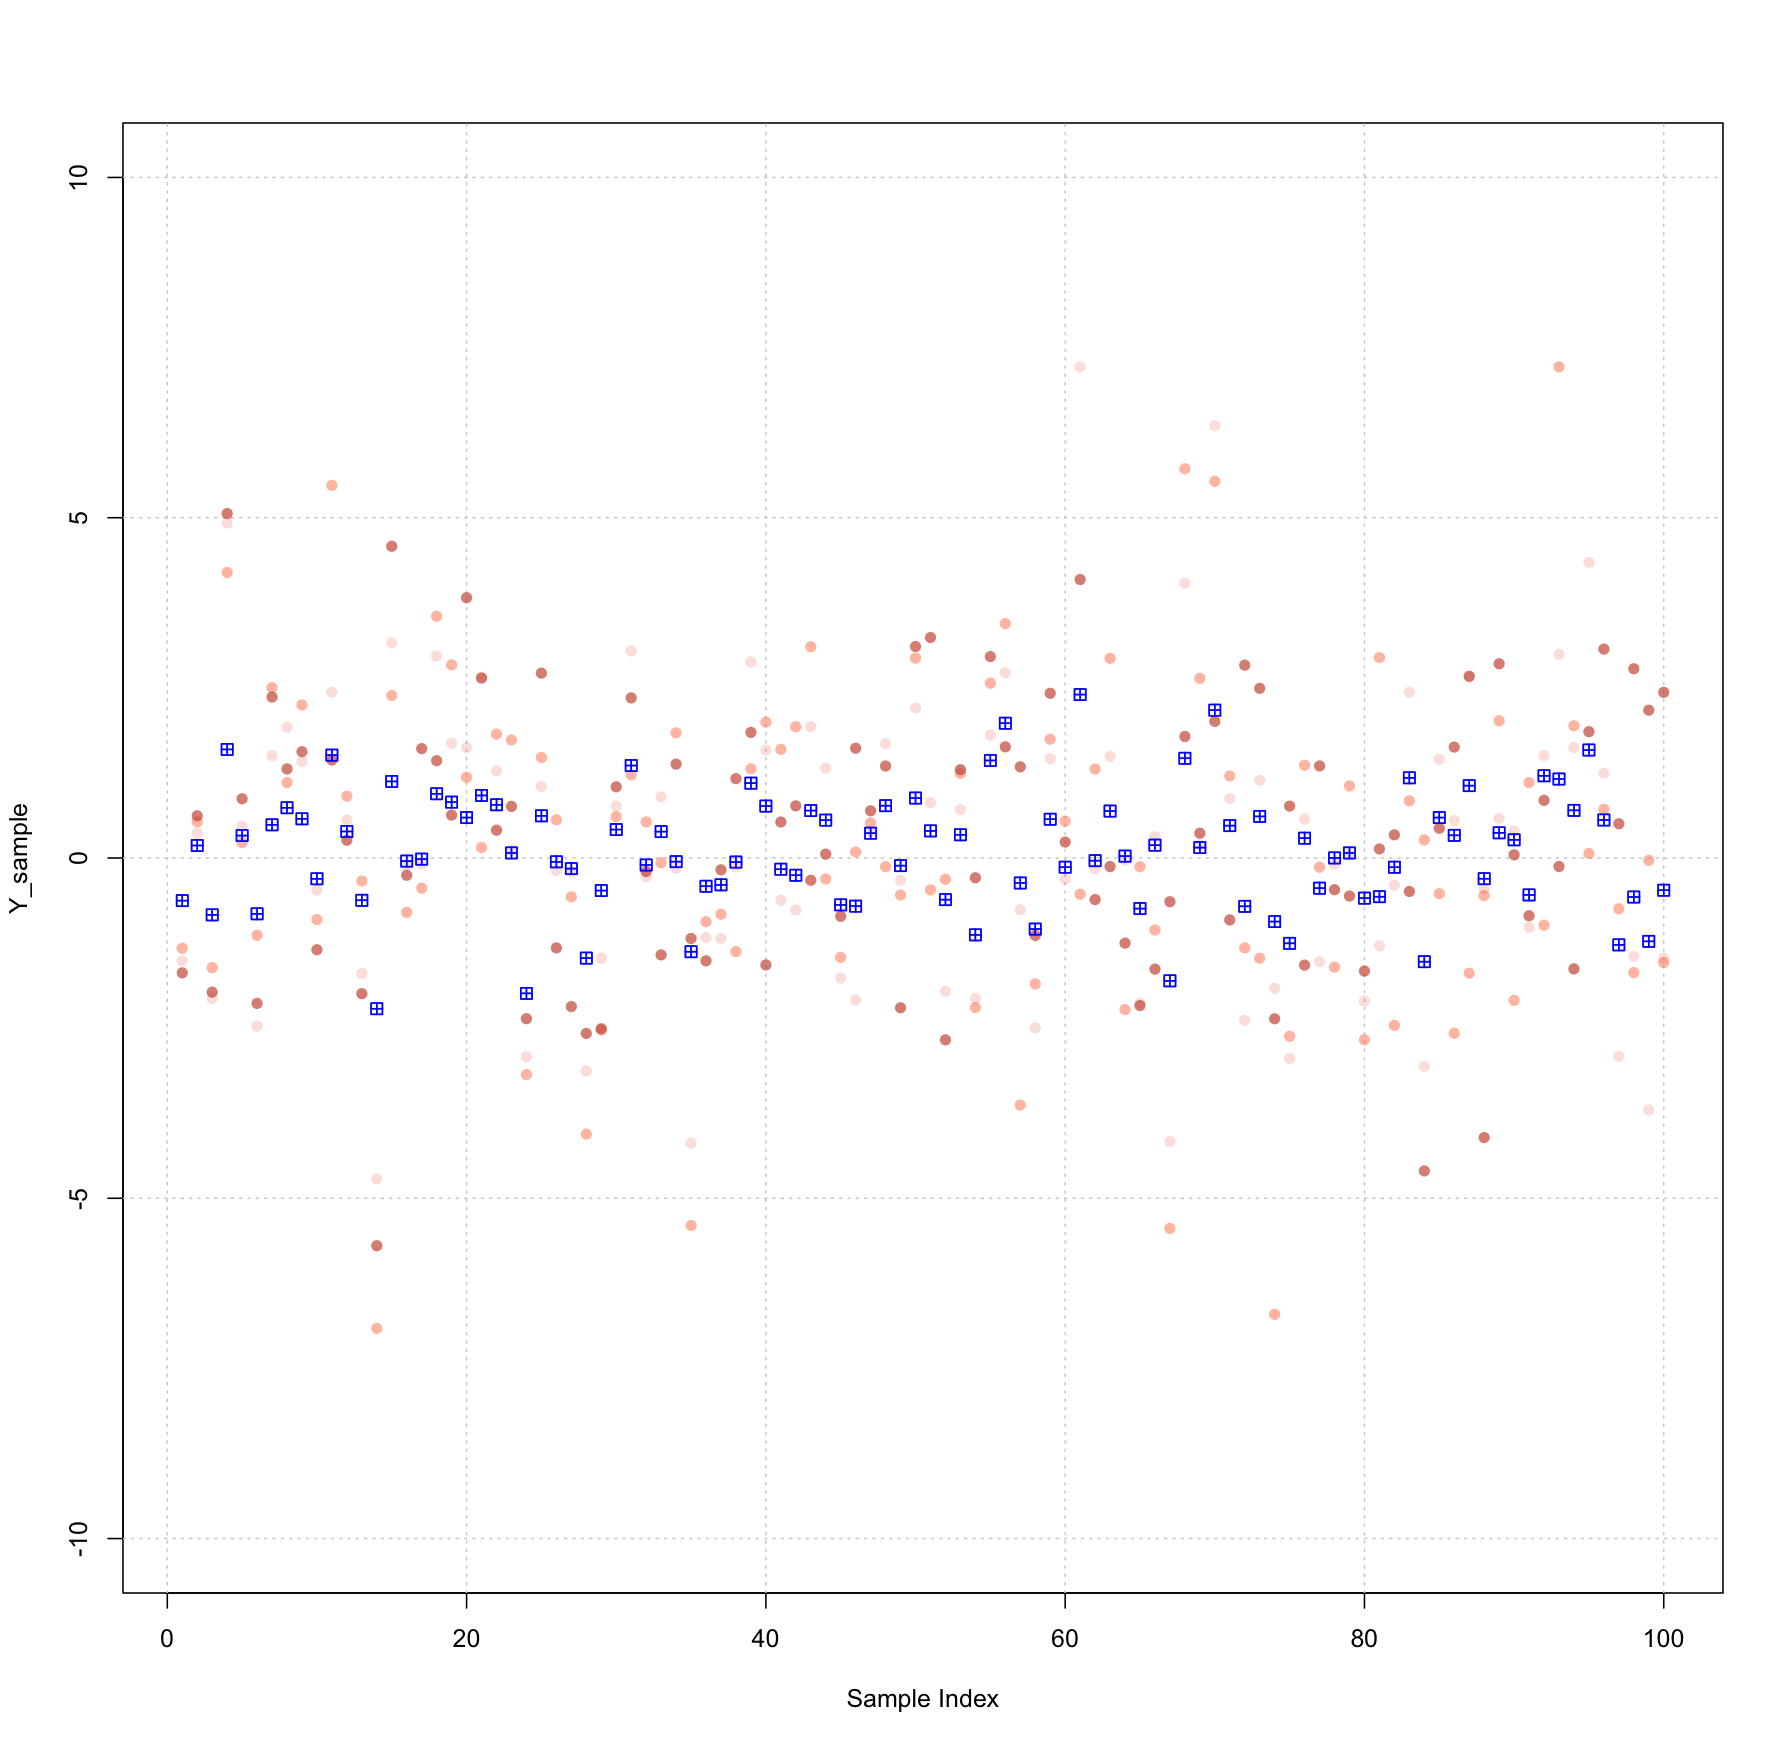
\includegraphics[scale=0.18]{image.png}}
\end{figure}
The blue squares are samples from an identity matrix sigma and others are from correlated sigmas.

\section*{Q2}
\subsection*{(a)}
\subsection*{(b)}
\subsection*{(c)}
\subsection*{(d)}
 
\end{document}  